\section{Lecture 12: Impulse Response and Convolution}



\subsection{Introduction}

In the previous sessions, we have studied various properties of Discrete Systems. Two of these properties when combined are of great analytical importance and hence of great help. These are, Linearity and Shift Invariance.

In this session, we look at the combination of the above two systems, names as Linear Shift Invariant systems. 

\subsection{A Linear Shift Invariant System}
Consider a system "S" which is Linear Shift Invariant. We have already studied that $$ Linearity = Additivity + Homogeneity$$
Thus, a Linear Shift Invariant System will have the properties of:
\begin{enumerate}
\item Additivity
\item Homogeneity
\item Shift Invariance
\end{enumerate}

In order to study the various input-output characteristics of a Linear Shift Invariant System, we could apply a certain known input function namely a 'Unit Impulse Response' Sequence. 


\subsubsection{Unit Impulse Response}
An impulse is a sudden, shortlived phenomenon.

A Unit Impulse Response sequence can be defined as the sequence which has just one finite value '1' at the origin and 'zero' else where.

Mathematically it can be written as:
$$ \delta[n] = 1, n=0$$
$$ \delta[n] = 0, n \neq 0 $$

\subsubsection{Taxation system as a Linear Shift Invariant System}
we had earlier seen the taxation system. We had the tax collected as Y[n] given by
$$Y[n] = { \alpha.X[n] +\beta. X[n-1] }$$
\subsubsection{Additivity}
We have already proven that the given system is Additive in the previous session. 

Now, in order to find out if the given system is Linear Shift Invariant, we need to check for Homogeneity as well as Shift Invariance.

\subsubsection{Homogeneity}
In order to prove that the system is Homogenous, we can scale the input $X[n]$ by a constant $\gamma$

$$X[n] = \gamma.X[n]$$
Therefore, $$Y[n] = { \alpha.X[n] +\beta. X[n-1] }$$
$$Y[n] = { \alpha.\gamma.X[n] +\beta.\gamma. X[n-1] }$$
$$Y[n] = \gamma .({ \alpha.X[n] +\beta. X[n-1] })$$
$$Y[n] = \gamma.Y[n]$$

Hence we prove that the Tax system is Homogenous.

\subsubsection{Shift Invariance}
To prove that the system is Shift Invariant, we Shift the input by an integer'D'.

$$X[n] = X[n-D]$$
Therefore, $$Y[n] = { \alpha.X[n] +\beta. X[n-1] }$$
$$Y[n] = { \alpha.X[n-D] +\beta. X[n-1-D] }$$
$$Y[n] = Y[n-D]$$

Thus we can see that the Taxation System is
\begin{itemize}
\item Additive
\item Homogenous
\item Shift Invariant
\end{itemize}

The Taxation System is thus found out to be an example of a 'Linear Shift Invariant' System.

\begin{figure}
\centering
\end{figure}





\subsubsection{Unit Impulse Response of a Linear Shift Invariant System}
Consider a Unit Impulse Sequence given as an input to a Linear Shift Invariant System. 
Input is given as $\delta[n]$
Therefore, $$Y[n] = { \alpha\delta[n] +\beta \delta[n-1] }$$
Now, we know that $\delta[n]=1 at n=0$
Hence we find that
$$Y[n]=\alpha $$ n=0
$$Y[n]=\beta $$ n-1=0 or n=1
$$Y[n]=0 $$ $n \neq 0$

Thus the tax collected or the output Y[n] will have only two discrete values. 

We thus analyze the unit impulse response of a Linear Shift Invariant System. 



\subsection{Theorem}
The theorem for Discrete Linear Time Invariant System states that 'the unit impulse response characterizes the system completely.

The above theorem states that given the unit impulse response of a system, it is possible to determine the output Y[n] for an input X[n].
 

\pagebreak

\chapter{The Impulse Response for Discrete LSI Systems}

\setcounter{section}{0}

\subsection{Introduction}
The input output relation of a Linear Time Invariant system can be found out if we know it's unit impulse response. 

We have formally stated this in a theorem that 'the unit impulse response characterizes the system completely.' 

We will look at the proof of the above theorem in this session.

\subsection{Proof of the Theorem}
Considering the theorem, we can say that we know that for a given LSI System for a given input $ X[n]=\delta[n]$ the output will be $Y[n]=h[n]$.

We shall now look at the proof step by step:


\subsubsection{Linear Combination of a Sequence}
Consider an input sequence

$$X[n]= [3, 2, -4, 7]$$
Consider 2 as the sample at the origin.


Thus, $X[-1]=3, X[0]=2, X[1]=-4, X[2]=7$.

The above sequence can be written as a combination of unit impulses of different magnitudes.

$$ X[n]= 3\delta[n+1] + 2\delta[n] - 4\delta[n-1] + 7\delta[n-2]$$
Therefore, 
$$ X[n]= X[n+1]\delta[n+1] + X[n]\delta[n] - X[n-1]\delta[n-1] + X[n-2]\delta[n-2]$$
$$X[n]=\sum_{k=-\infty}^{\infty} x[k]\delta[n-k]$$

\subsubsection{Shift Invariance}
We will now recall the properties of a LSI System. 
$X[n]=\delta[n]$
Since given system is Shift Invariant,
$\delta[n-D]\rightarrow h[n-D]$

\subsubsection{Homogeneity}
A LSI System is Homogeneous.
For a given value of $k$, the value of $X[k]$ will be constant.
scaling the impulse, shifted input by $X[k]$
Thus, $$X[k]\delta[n-k]\rightarrow X[k]h[n-k]$$

\subsubsection{Additivity}
LSI System shows the property of Additivity. 
$$\sum_{k=-\infty}^{\infty} X[k]\delta[n-k]\rightarrow \sum_{k=-\infty}^{\infty} X[k]h[n-k]$$


The term $'\sum_{k=-\infty}^{\infty} x[k]*\delta[n-k]'$ is nothing but $X[n]$ as seen above.

We can now conclude that the output of the system will be definitely known because of the earlier 3 properties discussed.

Therefore,$$Y[n]=\sum_{k=-\infty}^{\infty} X[k].h[n-k]$$

Hence we prove the theorem "constructively". That is, we now constructively and definitively know the input-output relation once we know the impulse response of the given LSI system.

\subsection{Introduction to Convolution}
The previously obtained output $Y[n]$ is obtained by 'convoluting' $X[n]$ and $h[n-k]$. 

This operation that is carried out between the two sequences is known as convolution. 

\pagebreak
\chapter{Discrete Convolution}

\setcounter{section}{0}

\subsection{Introduction}

Earlier we saw the concept of Convolution of two Sequences of Signals. 

Convolution is basically an operation between the two sequences which enables us to find out the output sequence. 

\subsection{Definition}
Convolution can be strictly defined as the operation between the input signal $X[n]$ and the impulse response $h[n]$ that results in the output $Y[n]$

$$Y[n]=X[n]*h[n]$$
In the above form, the $'*'$ term denotes Convolution. 
Therefore, $$Y[n]=\sum_{k=-\infty}^{\infty} X[k].h[n-k]$$


Note: The symbol $*$ will henceforth always refer to Convolution of two signals and NOT just simple multiplication.

\subsection{Procedure for Convolution}
\subsubsection{Applying the Input Signal}

\begin{figure}[ht]
\centering
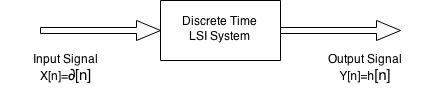
\includegraphics[width=0.5\textwidth]{Block.jpg}
\caption{\label{Step 1:} Applied input $X[n]=\delta[n]$}
\end{figure}


\subsubsection{Delaying the Input Signal}

\begin{figure}[ht]
\centering
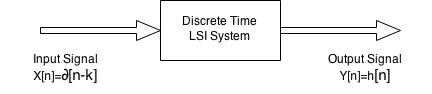
\includegraphics[width=0.5\textwidth]{Block_delay.jpg}
\caption{\label{Step 2:} Applied delay to the signal}
\end{figure}
\pagebreak



\subsubsection{Scaling the delayed Input Signal}

\begin{figure}[ht]
\centering
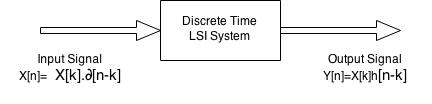
\includegraphics[width=0.5\textwidth]{Block_scale.jpg}
\caption{\label{Step 3:} Scaling the input by X[k]}
\end{figure}

\subsubsection{Adding the Scaled Impulses over the entire Range}

\begin{figure}[ht]
\centering
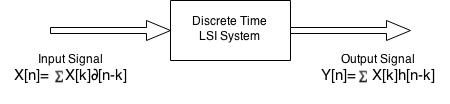
\includegraphics[width=0.5\textwidth]{Block_sum.jpg}
\caption{\label{Step 4:} Summing the input over the entire region}
\end{figure}


\subsection{Applications}
A few Applications of Convolution are listed below:
\begin{itemize}
\item To obtain the response (or output) signal of the discrete time signal input applied.
\item To obtain overall impulse response signal $h[n]$ for interconnected systems.
\item To determine similarity (co-relation) between the transmitted and reflected (or received) signal.This is also called as Auto-Corelation.
\item To obtain similarity between 2 different signals. Also called Cross-Corelation. 
\end{itemize}


\subsection{Examples on Convolution}
\subsubsection{Example 1:}

Calculate the output Y[1] for 
$$X[n]=[3,1,2]\hspace{10mm}X[0]=3$$
$$h[n]=[3,0,2]\hspace{10mm}X[0]=3$$

To find out $Y[1]$, replace $n$ by 1 in the Convolution formula.

$$Y[1]=\sum_{k=-\infty}^{\infty} X[k].h[1-k]$$

The signal sequence $h[1-k]$ will be represented as:
$$h[1-k]=[2,0,3]\hspace{10mm}h[0]=0$$

While Convoluting 2 sequences, as we have seen in Continuous Time domain, we need to find the part of the signal sequences that overlap. 

Therefore,
$$Y[1]=(X[0].h[o])+(X[1].h[1])$$
$$Y[1]=(3.0)+(1.3)$$
$$Y[1]=3$$

Thus we Convolve the signal sequences $X[n]$ and $h[n]$ in order to find the output $Y[n]$ at the point $n=1$.

\subsection{Properties of Convolution}
\subsubsection{Commutativity}
If, $$Y[n]=X[n]*h[n]$$

Then, by the Commutative Property of Convolution, 
$$Y[n]=h[n]*X[n]$$

\subsubsection{Distributivity}

If, $$Y[n]=X[n]*(h_1[n]+h_2[n])$$

Then, by the Distributive Property of Convolution, 
$$Y[n]=X[n]*h_1[n]+X[n]*h_2[n]$$

\subsubsection{Associativity}

If, $$Y[n]=X[n]*(h_1[n]*h_2[n])$$

Then, by the Associative Property of Convolution, 
$$Y[n]=(X[n]*h_1[n])*h_2[n]$$





